\section{Anexo}

\subsection{Circuito Esquemático}

\begin{figure}[H]
    \centering
    % Controla la altura máxima para no empujar el título
    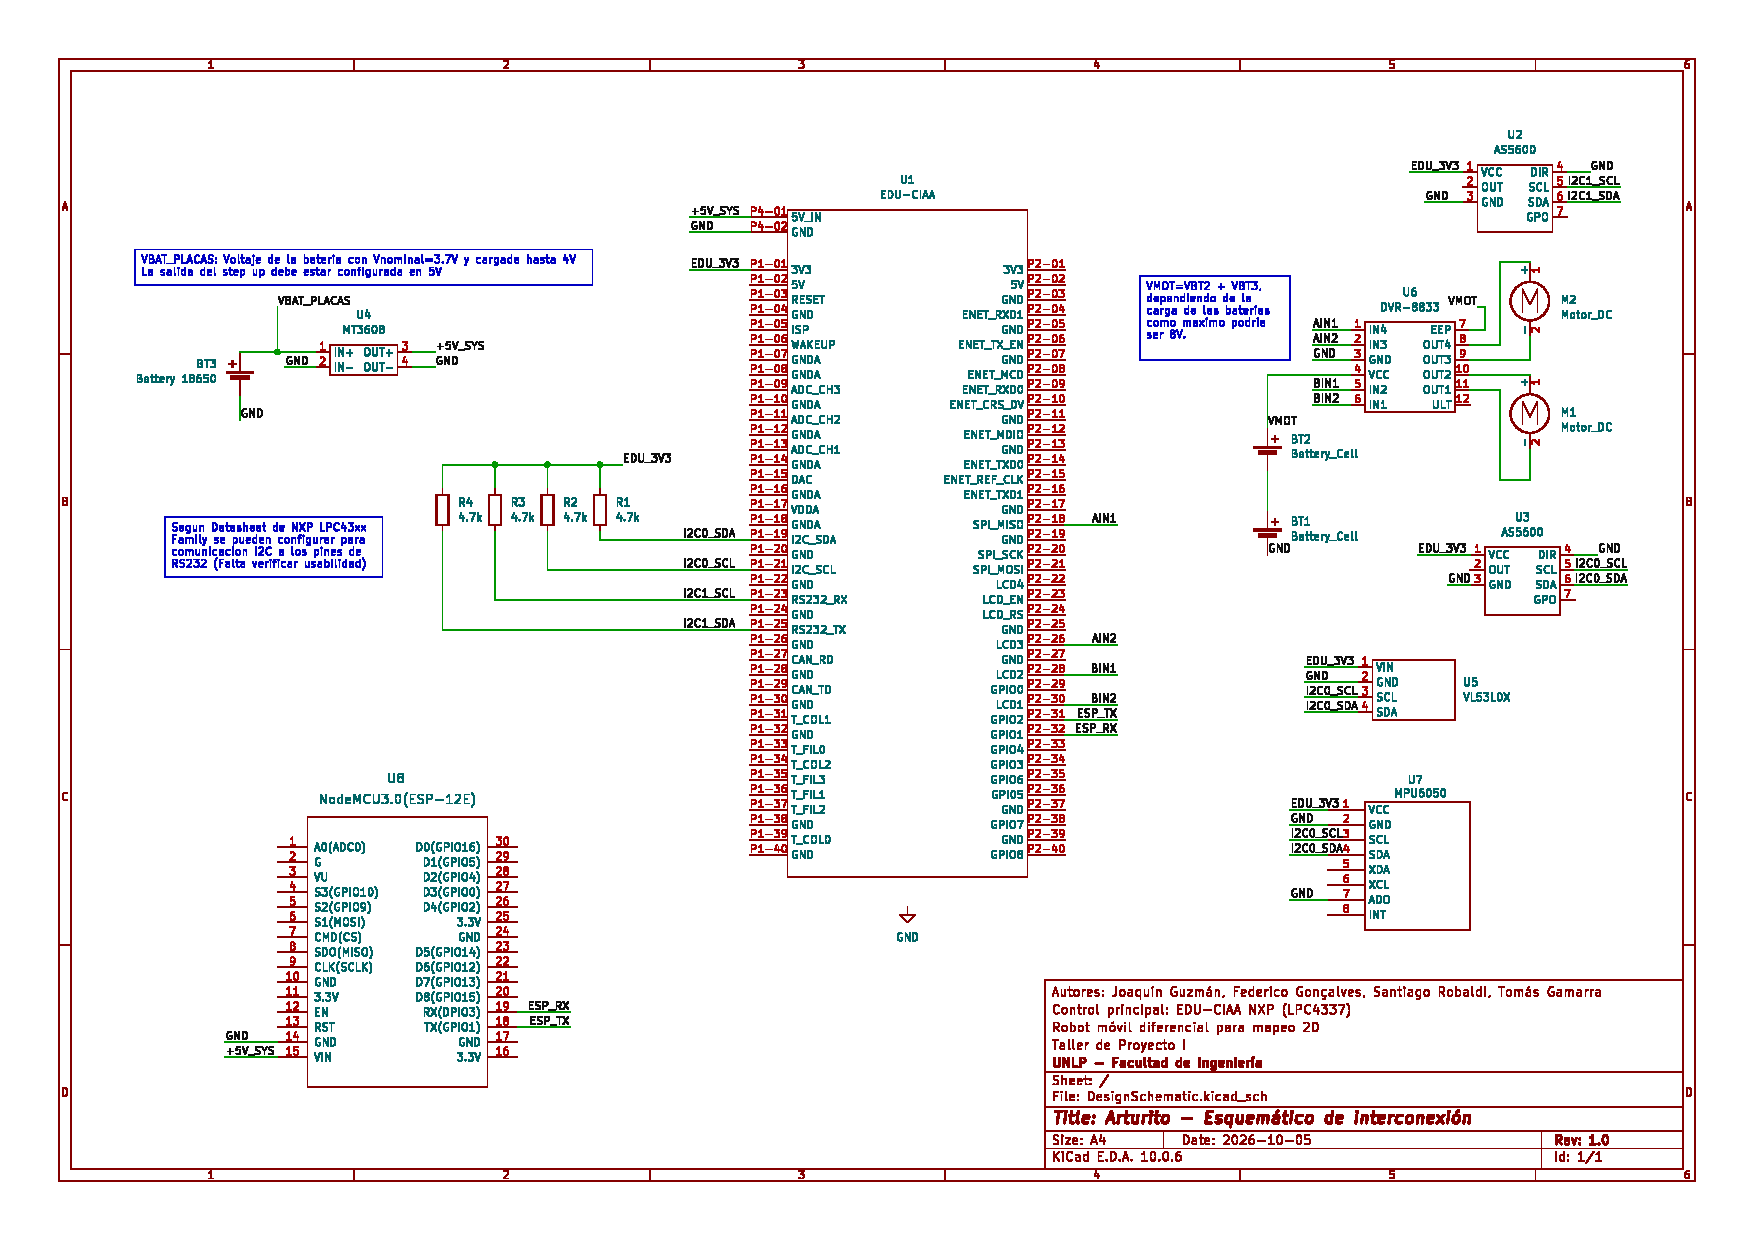
\includegraphics[width=\textwidth, height=0.75\textheight, keepaspectratio]{Esquematico.pdf}
    \caption{Esquemático completo del sistema de control y potencia.}
    \label{fig:esquematico_anexo}
\end{figure}

% ------------------------------------------------------------------------------
\subsection{Lista de materiales (BOM)}
% ------------------------------------------------------------------------------
\begin{table}[H]
\centering
\caption{Lista de materiales preliminar.}
\label{tab:bom}
\small
\begin{tabular}{cL{5.6cm}L{1.6cm}L{3cm}}
\toprule
Ítem & Descripción / código de parte & Cant. & Formato \\
\midrule
1 & Motorreductor GA12-N20 (Handson Technology), \SI{6}{V}--\SI{12}{V}, 150:1 & 2 & Motor con caja metálica \\
2 & Módulo driver DRV8833 & 1 & Módulo, pines 2,54~mm \\
3 & Módulo elevador MT3608 (\SI{5}{V}, ramal de lógica) & 1 & Módulo \\
4 & Celda Li-ion 18650, \SI{3,7}{V} (capacidad a confirmar) & 3 & Cilíndrica \\
5 & Portapilas 18650: uno de 1 celda y uno de 2 celdas en serie & 2 & Portapilas \\
6 & Protección de celdas (BMS), no definida & \pq & \pq \\
7 & Cargador de celdas, no definido & \pq & \pq \\
8 & Capacitor electrolítico \SI{470}{\micro F}/\SI{16}{V} & 1 & Componente discreto \\
9 & Capacitor cerámico \SI{100}{nF} (104) & 2 & Componente discreto \\
10 & ESP32 DevKit v1 & 1 & Módulo \\
11 & IMU MPU6050 & 1 & Módulo \\
12 & Módulo sensor de distancia VL53L0X & 1 & Módulo \\
13 & Módulo AS5600 (TinyTronics AS5600MOD), con imán diametral incluido & 2 & Módulo \SI{23}{mm}$\times$\SI{23}{mm} \\
14 & Ruedas de \SI{44}{mm} de diámetro & 2 & Rueda plástica / goma \\
\midrule
15 & Filamento ABS (para impresión 3D de piezas estructurales) & \SI{1}{kg} & Carrete de filamento \\
16 & Chasis inferior (nivel base para motores, celdas y sensores) & 1 & Pieza impresa (ABS) \\
17 & Chasis superior modular para prototipado (soporte de \emph{breadboard}) & 1 & Pieza impresa (ABS) \\
18 & Chasis superior modular (soporte para placa EDU-CIAA) & 1 & Pieza impresa (ABS) \\
19 & Varilla roscada M6 de \SI{1}{m} & 1 & Varilla \\
20 & Tuercas hexagonales M6 & 20 & Tornillería \\
21 & Tornillos M3 & 6 & Tornillería \\
22 & Tuercas hexagonales M3 & 6 & Tornillería \\
23 & Apoyo trasero: patín impreso en ABS (o \emph{ball caster} de acero) & 1 & Pieza impresa / Comp. \\
\bottomrule
\bottomrule
\end{tabular}
\end{table}
\pendiente{confirmar cantidades y qué materiales ya se poseen, como la EDU-CIAA y los motores del prototipo.}